
\section{Soluciones y griegas}


\subsection{Griegas}
\begin{center}
    \begin{tabularx}{\textwidth}{|c|X|}
        \hline
        \textbf{Delta} $\Delta = \frac{\partial V}{\partial S}$ &  Lo que se tiene que comprar/vender en cada momento según el valor del subyacente para mantener la cartera libre de riesgo. \\
        \hline
        \textbf{Gamma} $\Gamma = \frac{\partial^2 V}{\partial S^2}$ & Es una medida de cuánto y cuantas veces se tiene que \textit{rehedged} para mantener la cartera libre de riesgo. \\
        \hline
        \textbf{Theta} $\Gamma = \frac{\partial V}{\partial t}$ & Contribuye a que la cartera gane el interés correspondiente. \\
        \hline
        \textbf{Speed} $\frac{\partial V}{\partial t}$ & Como gamma, pero para mayor precisión. \\
        \hline
        \textbf{Vega} $\frac{\partial V}{\partial \sigma}$ & ?? \\
        \hline
    \end{tabularx}
\end{center}



\subsection{Tablas de soluciones}
\begin{center}
    \begin{tabularx}{\textwidth}{|X|X|X|}
        \hline
         & \textbf{Call} & \textbf{Put} \\
         \hline
         \textbf{Value (Black-Scholes value)} &  $S e^{-D(T-t)} N(d_1) - E e^{-r(T-t)} N(d_2)$  &  $-S e^{-D(T-t)} N(-d_1) + E e^{-r(T-t)} N(-d_2)$  \\
        \hline
         \textbf{Delta } $\left( \frac{\partial V}{\partial S} \right)$ & $ e^{-D(T-t)} N(d_1) $ & $ e^{-D(T-t)} (N(d_1) - 1) $ \\
         \hline
        \textbf{Gamma } $\left( \frac{\partial^2 V}{\partial S^2} \right)$ & $ \frac{e^{-D(T-t)} N'(d_1)}{\sigma S \sqrt{T - t}} $ & $ \frac{e^{-D(T-t)} N'(d_1)}{\sigma S \sqrt{T - t}} $ \\
        \hline
        \textbf{Theta } $\left( \frac{\partial V}{\partial t} \right)$ & $ -\frac{\sigma S e^{-D(T-t)} N'(d_1)}{2 \sqrt{T - t}} + D S N(d_1) e^{-D(T-t)} - r E e^{-r(T-t)} N(d_2) $ & $ -\frac{\sigma S e^{-D(T-t)} N'(-d_1)}{2 \sqrt{T - t}} - D S N(-d_1) e^{-D(T-t)} + r E e^{-r(T-t)} N(-d_2) $ \\
        \hline
        \textbf{Speed } $\left( \frac{\partial^3 V}{\partial S^3} \right)$ & $ -\frac{e^{-D(T-t)} N'(d_1)}{\sigma^2 S^2 (T - t)} (d_1 + \sigma \sqrt{T - t}) $ & $ -\frac{e^{-D(T-t)} N'(d_1)}{\sigma^2 S^2 (T - t)} (d_1 + \sigma \sqrt{T - t}) $ \\
        \hline
        \textbf{Vega } $\left( \frac{\partial V}{\partial \sigma} \right)$ & $ S \sqrt{T - t} e^{-D(T-t)} N'(d_1) $ & $ S \sqrt{T - t} e^{-D(T-t)} N'(d_1) $ \\
        \hline
        \textbf{Rho } $\left( \frac{\partial V}{\partial r} \right)$ & $ E (T - t) e^{-r(T-t)} N(d_2) $ & $ -E (T - t) e^{-r(T-t)} N(-d_2) $ \\
        \hline
        \textbf{Rho } $\left( \frac{\partial V}{\partial D} \right)$ & $ -(T - t) S e^{-D(T-t)} N(d_1) $ & $ (T - t) S e^{-D(T-t)} N(-d_1) $ \\
        \hline
    \end{tabularx}
\end{center}
\begin{align*}
    d_1 &= \frac{\log \left( \frac{S}{E} \right) + \left( r - D + \frac{1}{2} \sigma^2 \right) (T - t)}{\sigma \sqrt{T - t}} && N(x) = \frac{1}{\sqrt{2 \pi}} \int_{-\infty}^x e^{- \frac{1}{2} y^2} \, dy \\
    d_2 &= d_1 - \sigma \sqrt{T - t} &&  N'(x) = \frac{1}{\sqrt{2 \pi}} e^{- \frac{1}{2} x^2}
\end{align*}

\begin{center}
    \begin{tabularx}{\textwidth}{|X|X|X|}
        \hline
        & \textbf{Binary Call} & \textbf{Binary Put} \\
        \hline
        \textbf{Value (Black-Scholes value)} & $ e^{-r(T-t)} N(d_2) $ & $ e^{-r(T-t)} (1 - N(d_2)) $ \\
        \hline
        \textbf{Delta } & $ \frac{e^{-r(T-t)} N'(d_2)}{\sigma S \sqrt{T - t}} $ & $ -\frac{e^{-r(T-t)} N'(d_2)}{\sigma S \sqrt{T - t}} $ \\
        \hline
        \textbf{Gamma } $\left( \frac{\partial^2 V}{\partial S^2} \right)$ & $ -\frac{e^{-r(T-t)} d_1 N'(d_2)}{\sigma^2 S (T - t)} $ & $ \frac{e^{-r(T-t)} d_1 N'(d_2)}{\sigma^2 S (T - t)} $ \\
        \hline
        \textbf{Theta } $\left( \frac{\partial V}{\partial t} \right)$ & $ r e^{-r(T-t)} N(d_2) \left( \frac{d_1}{2 (T - t)} - \frac{r - D}{\sigma \sqrt{T - t}} \right) $ & $ r e^{-r(T-t)} (1 - N(d_2)) \left( \frac{d_1}{2 (T - t)} - \frac{r - D}{\sigma \sqrt{T - t}} \right) $ \\
        \hline
        \textbf{Speed } $\left( \frac{\partial^3 V}{\partial S^3} \right)$ & $ \frac{e^{-r(T-t)} N'(d_2)}{\sigma^2 S (T - t)} \left( -2 d_1 + \frac{1 - d_1 d_2}{\sigma \sqrt{T - t}} \right) $ & $ \frac{e^{-r(T-t)} N'(d_2)}{\sigma^2 S (T - t)} \left( -2 d_1 + \frac{1 - d_1 d_2}{\sigma \sqrt{T - t}} \right) $ \\
        \hline
        \textbf{Vega } $\left( \frac{\partial V}{\partial \sigma} \right)$ & $ -\frac{e^{-r(T-t)} N'(d_2) d_1}{\sigma \sqrt{T - t}} $ & $ \frac{e^{-r(T-t)} N'(d_2) d_1}{\sigma \sqrt{T - t}} $ \\
        \hline
        \textbf{Rho } $\left( \frac{\partial V}{\partial r} \right)$ & $ -(T - t) e^{-r(T-t)} N(d_2) + \frac{e^{-r(T-t)} N'(d_2)}{\sigma} $ & $ -(T - t) e^{-r(T-t)} (1 - N(d_2)) - \frac{e^{-r(T-t)} N'(d_2)}{\sigma} $ \\
        \hline
        \textbf{Rho } $\left( \frac{\partial V}{\partial D} \right)$ & $ \frac{\sqrt{T - t}}{\sigma} e^{-r(T-t)} N'(d_2) $ & $ -\frac{\sqrt{T - t}}{\sigma} e^{-r(T-t)} N'(d_2) $ \\
        \hline
    \end{tabularx}
\end{center}
\begin{align*}
    d_1 &= \frac{\log \left( \frac{S}{E} \right) + \left( r - D + \frac{1}{2} \sigma^2 \right) (T - t)}{\sigma \sqrt{T - t}} && N(x) = \frac{1}{\sqrt{2 \pi}} \int_{-\infty}^x e^{- \frac{1}{2} y^2} \, dy \\
    d_2 &= d_1 - \sigma \sqrt{T - t} &&  N'(x) = \frac{1}{\sqrt{2 \pi}} e^{- \frac{1}{2} x^2}
\end{align*}




\subsection{Representación gráfica de soluciones}
En este apartado se va a graficar cada una de las soluciones
\subsubsection{Call option}
\begin{figure}[H]
    \centering
    \begin{subfigure}[b]{0.35\linewidth}
        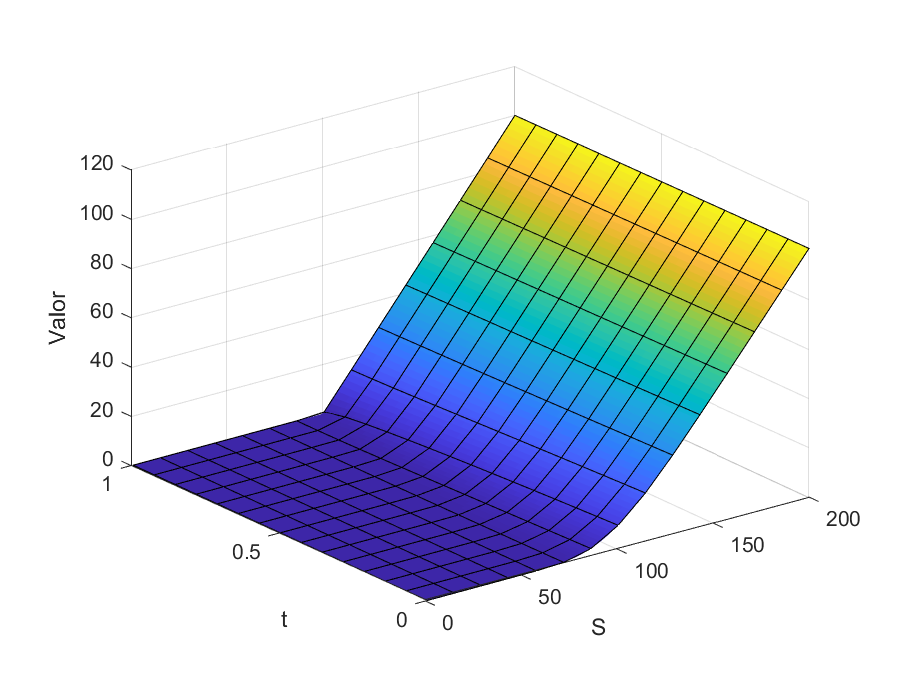
\includegraphics[width=\linewidth]{Imagenes/6_Sols/Call/Call3D.eps}
        \caption{Solución}
    \end{subfigure}
    \begin{subfigure}[b]{0.35\linewidth}
        \includegraphics[width=\linewidth]{Imagenes/6_Sols/Call/CallSFijo.eps}
        \caption{Solución con S fijo}
    \end{subfigure}
    \begin{subfigure}[b]{0.35\linewidth}
        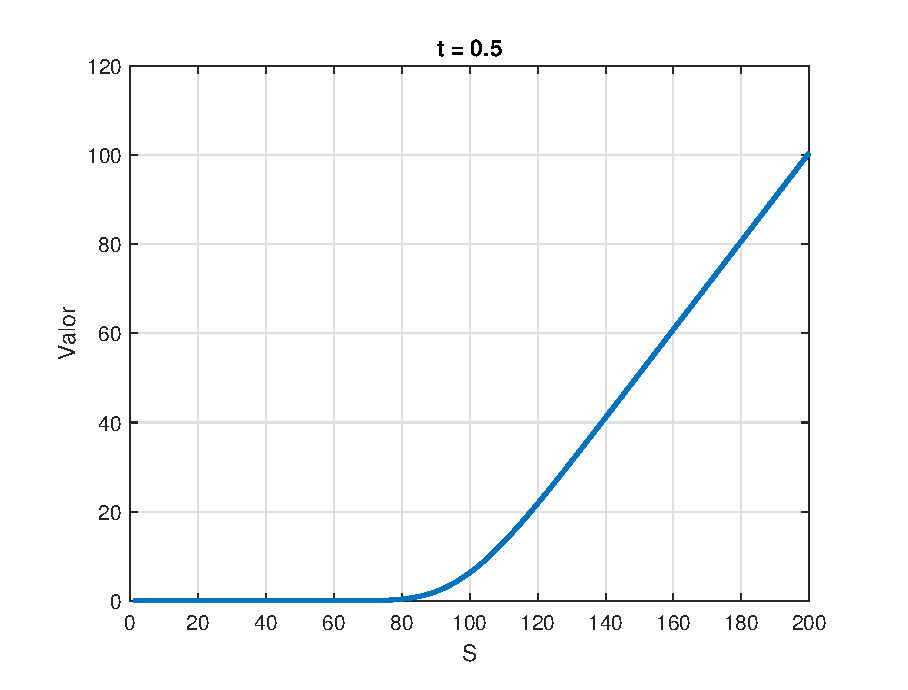
\includegraphics[width=\linewidth]{Imagenes/6_Sols/Call/CalltFIjo.eps}
        \caption{Solución con t fijo}
    \end{subfigure}
    \begin{subfigure}[b]{0.35\linewidth}
        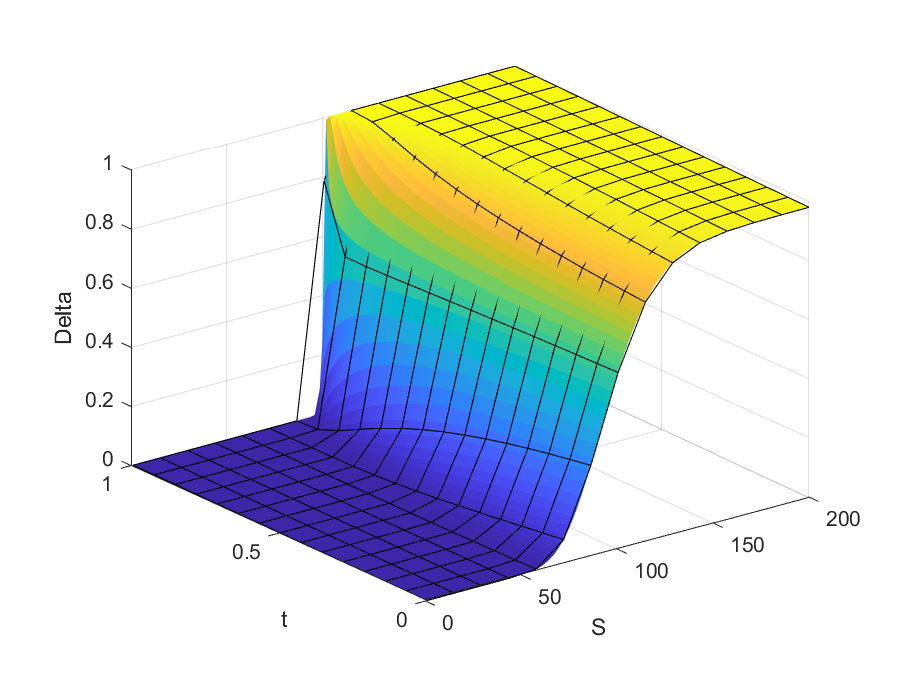
\includegraphics[width=\linewidth]{Imagenes/6_Sols/Call/Call_Delta.eps}
        \caption{Delta}
    \end{subfigure}
    \begin{subfigure}[b]{0.35\linewidth}
        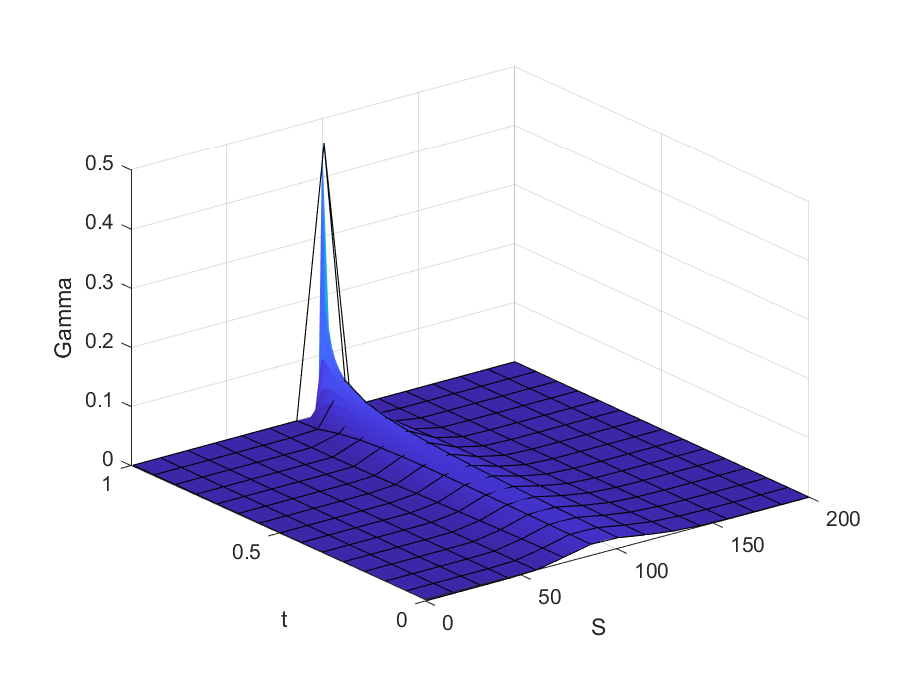
\includegraphics[width=\linewidth]{Imagenes/6_Sols/Call/Call_Gamma.eps}
        \caption{Gamma}
    \end{subfigure}
    \begin{subfigure}[b]{0.35\linewidth}
        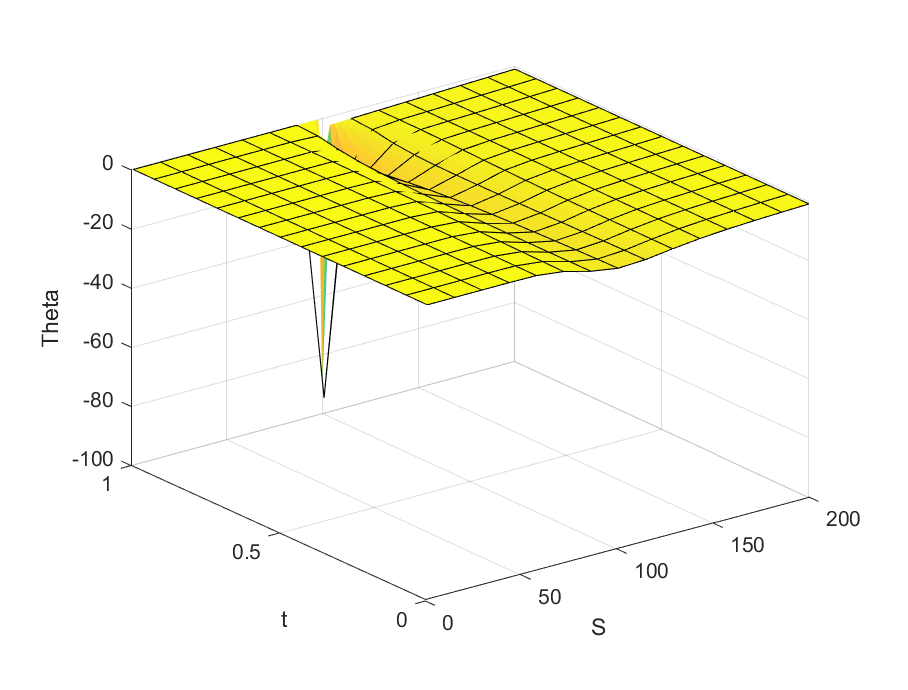
\includegraphics[width=\linewidth]{Imagenes/6_Sols/Call/Call_Theta.eps}
        \caption{Theta}
    \end{subfigure}
    \begin{subfigure}[b]{0.35\linewidth}
        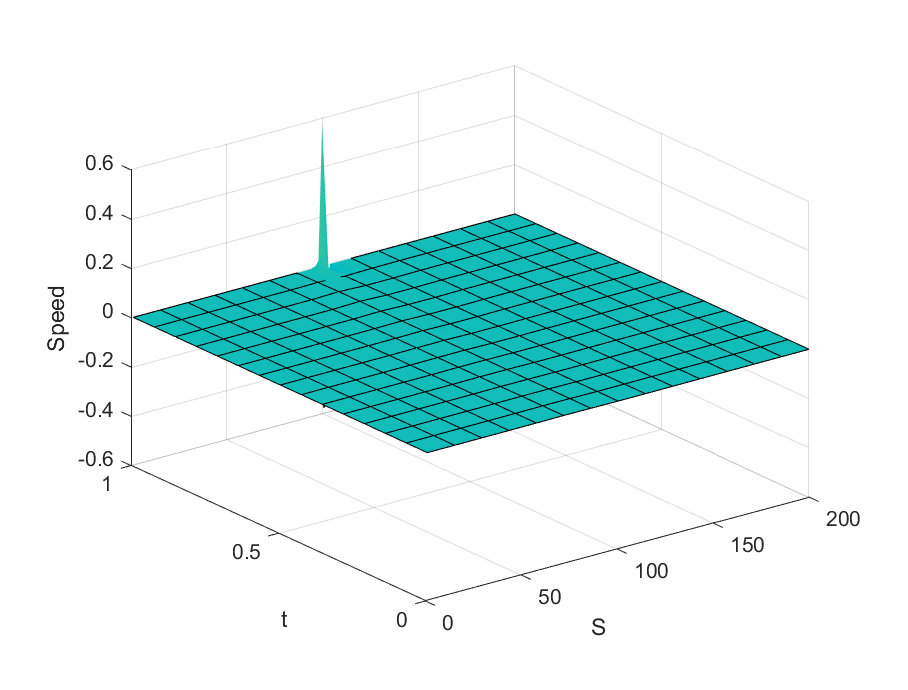
\includegraphics[width=\linewidth]{Imagenes/6_Sols/Call/Call_Speed.eps}
        \caption{Speed}
    \end{subfigure}
    \begin{subfigure}[b]{0.35\linewidth}
        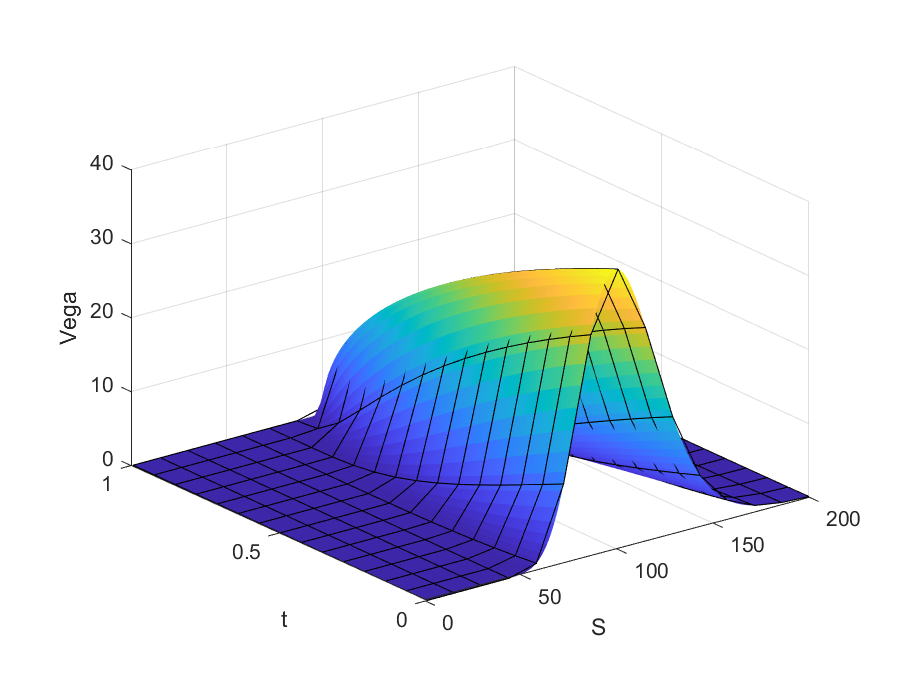
\includegraphics[width=\linewidth]{Imagenes/6_Sols/Call/Call_Vega.eps}
        \caption{Vega}
    \end{subfigure}
    \begin{subfigure}[b]{0.35\linewidth}
        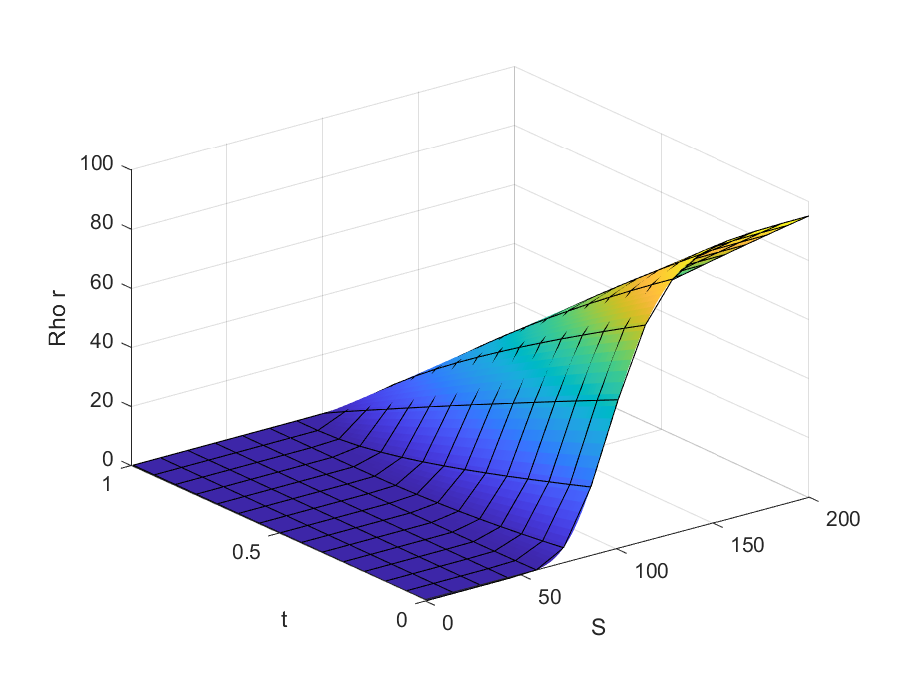
\includegraphics[width=\linewidth]{Imagenes/6_Sols/Call/Call_Rho_r.eps}
        \caption{Rho (r)}
    \end{subfigure}
    \begin{subfigure}[b]{0.35\linewidth}
        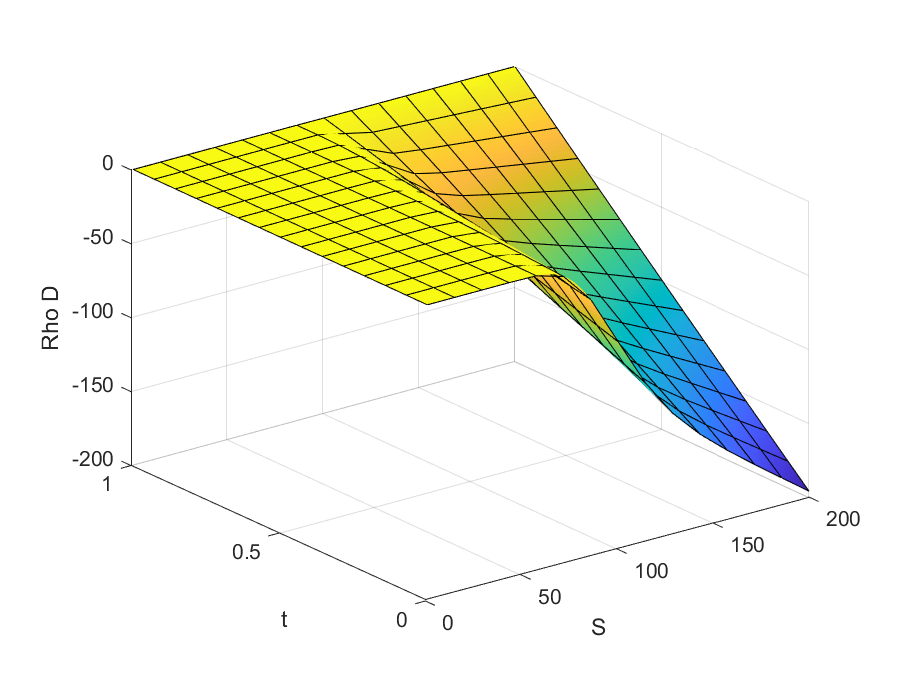
\includegraphics[width=\linewidth]{Imagenes/6_Sols/Call/Call_Rho_D.eps}
        \caption{Rho (D)}
    \end{subfigure}
\end{figure}


\subsubsection{Put option}
\begin{figure}[H]
    \centering
    \begin{subfigure}[b]{0.35\linewidth}
        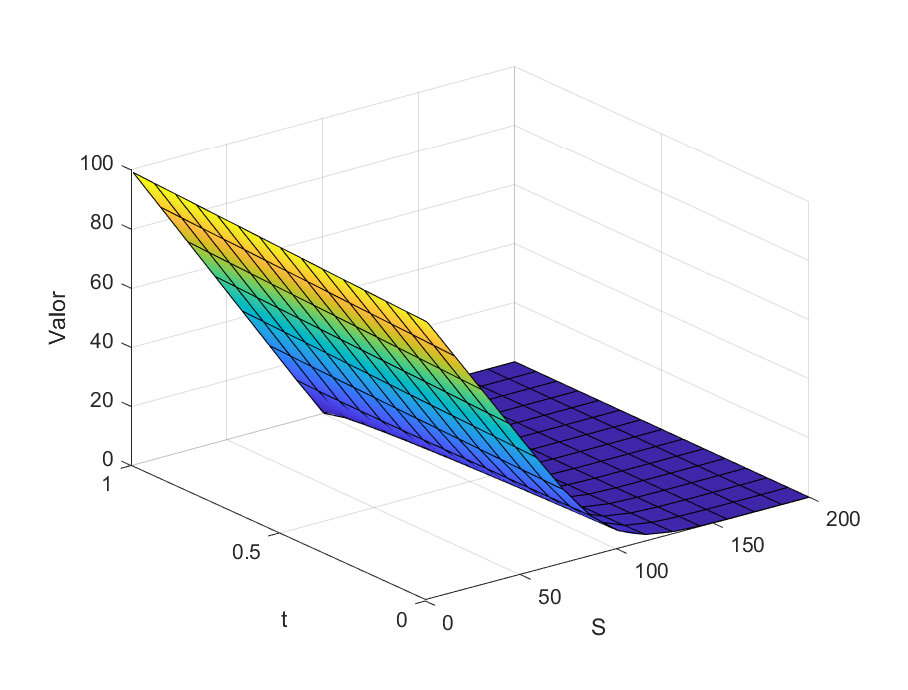
\includegraphics[width=\linewidth]{Imagenes/6_Sols/Put/Put3D.eps}
        \caption{Solución}
    \end{subfigure}
    \begin{subfigure}[b]{0.35\linewidth}
        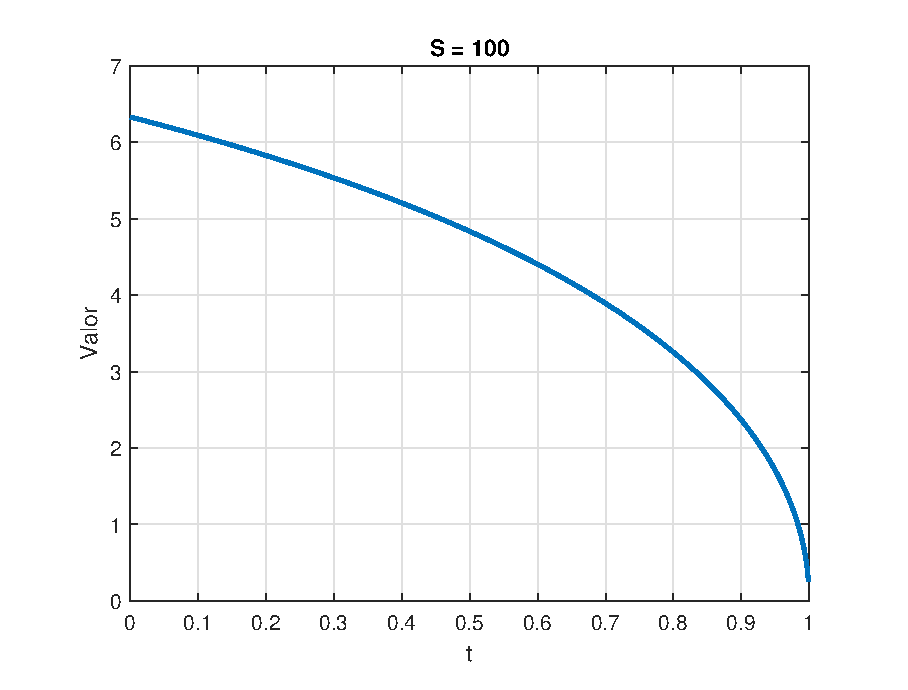
\includegraphics[width=\linewidth]{Imagenes/6_Sols/Put/PutSFijo.eps}
        \caption{Solución con S fijo}
    \end{subfigure}
    \begin{subfigure}[b]{0.35\linewidth}
        \includegraphics[width=\linewidth]{Imagenes/6_Sols/Put/PuttFIjo.eps}
        \caption{Solución con t fijo}
    \end{subfigure}
    \begin{subfigure}[b]{0.35\linewidth}
        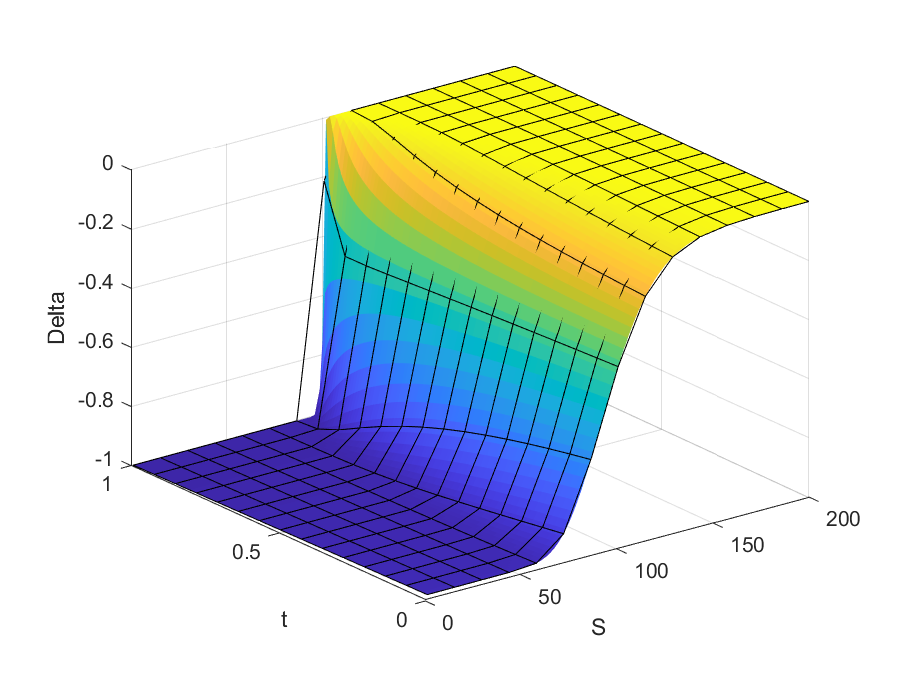
\includegraphics[width=\linewidth]{Imagenes/6_Sols/Put/Put_Delta.eps}
        \caption{Delta}
    \end{subfigure}
    \begin{subfigure}[b]{0.35\linewidth}
        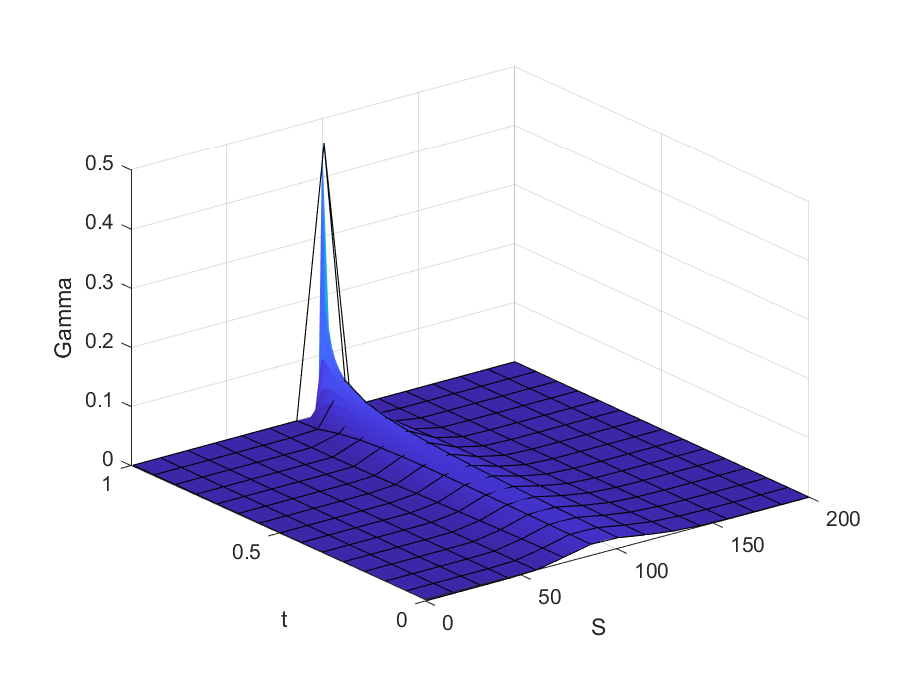
\includegraphics[width=\linewidth]{Imagenes/6_Sols/Put/Put_Gamma.eps}
        \caption{Gamma}
    \end{subfigure}
    \begin{subfigure}[b]{0.35\linewidth}
        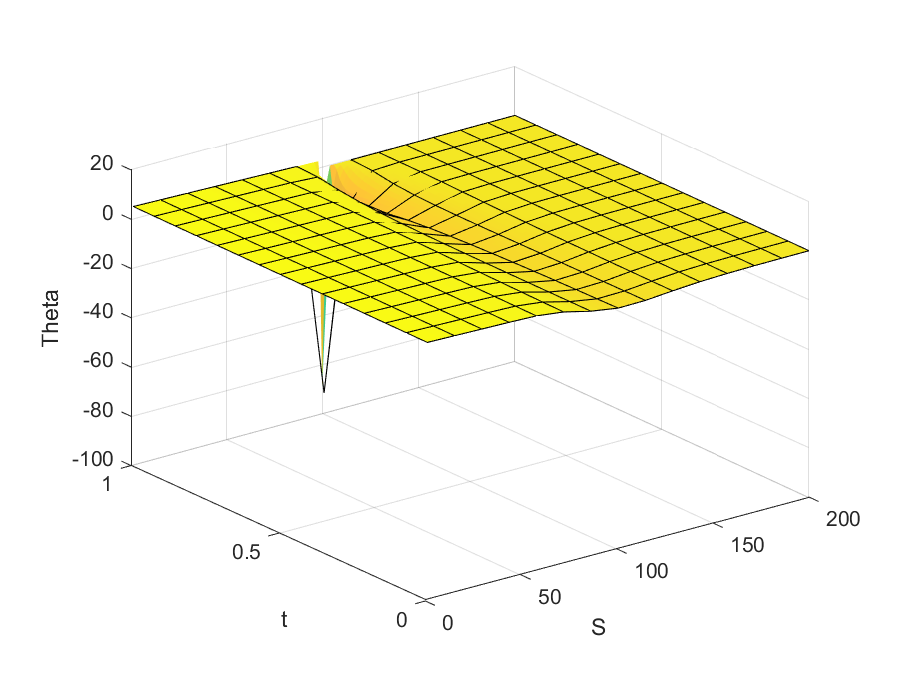
\includegraphics[width=\linewidth]{Imagenes/6_Sols/Put/Put_Theta.eps}
        \caption{Theta}
    \end{subfigure}
    \begin{subfigure}[b]{0.35\linewidth}
        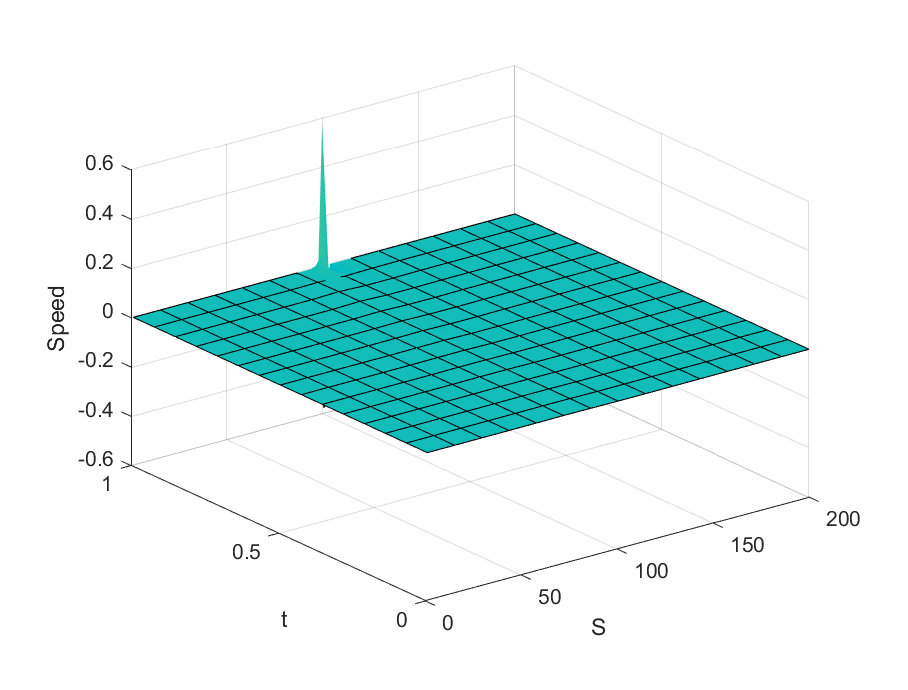
\includegraphics[width=\linewidth]{Imagenes/6_Sols/Put/Put_Speed.eps}
        \caption{Speed}
    \end{subfigure}
    \begin{subfigure}[b]{0.35\linewidth}
        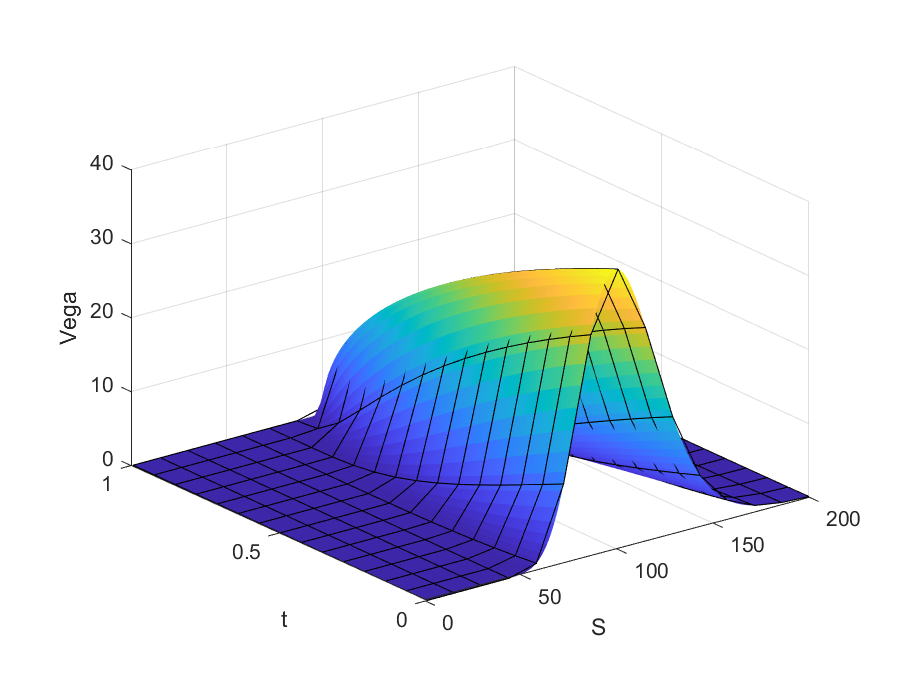
\includegraphics[width=\linewidth]{Imagenes/6_Sols/Put/Put_Vega.eps}
        \caption{Vega}
    \end{subfigure}
    \begin{subfigure}[b]{0.35\linewidth}
        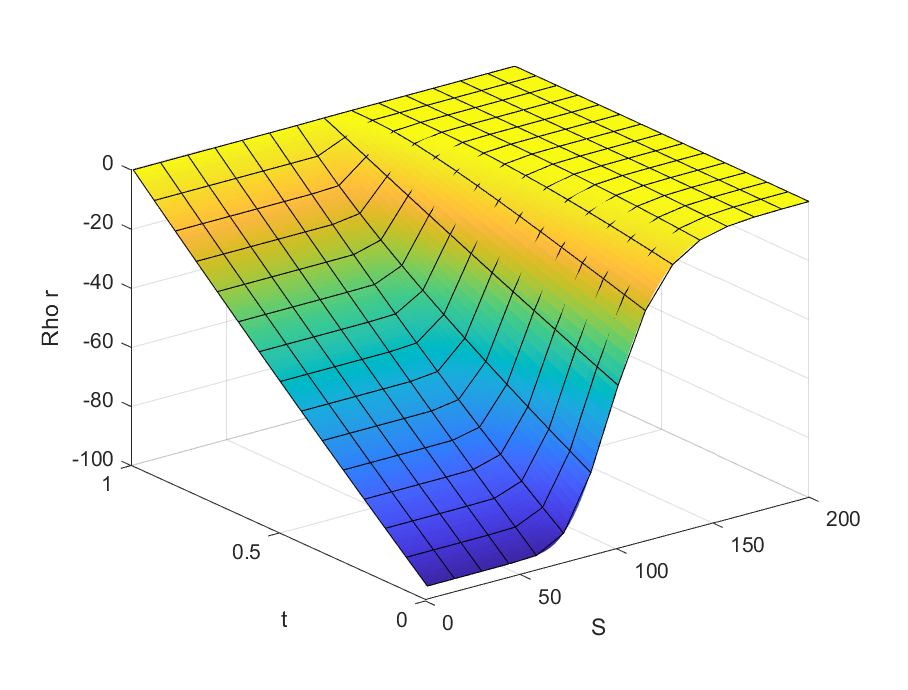
\includegraphics[width=\linewidth]{Imagenes/6_Sols/Put/Put_Rho_r.eps}
        \caption{Rho (r)}
    \end{subfigure}
    \begin{subfigure}[b]{0.35\linewidth}
        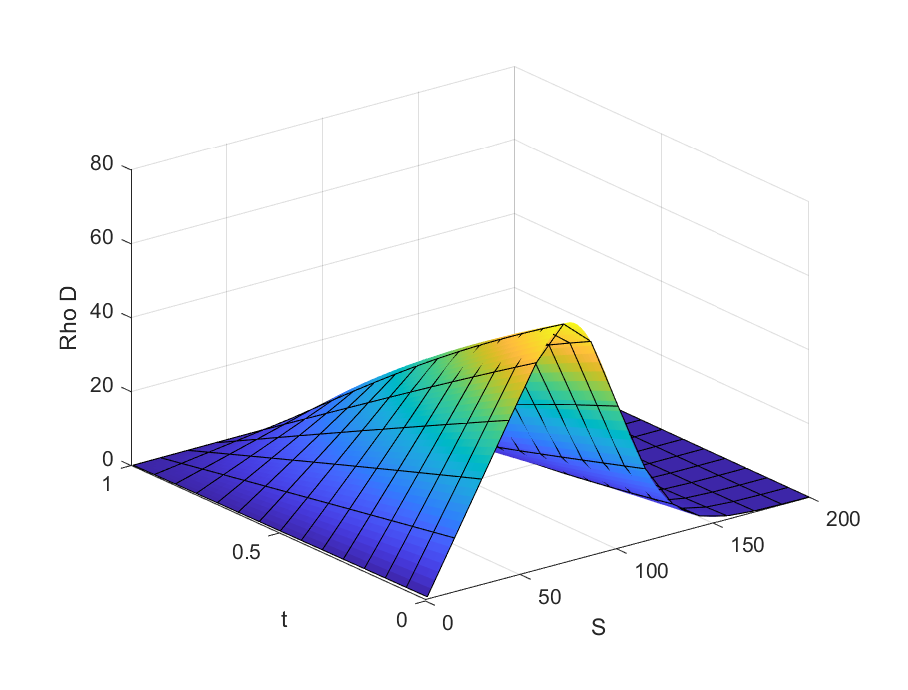
\includegraphics[width=\linewidth]{Imagenes/6_Sols/Put/Put_Rho_D.eps}
        \caption{Rho (D)}
    \end{subfigure}
\end{figure}



\subsubsection{Binary Call option}
\begin{figure}[H]
    \centering
    \begin{subfigure}[b]{0.35\linewidth}
        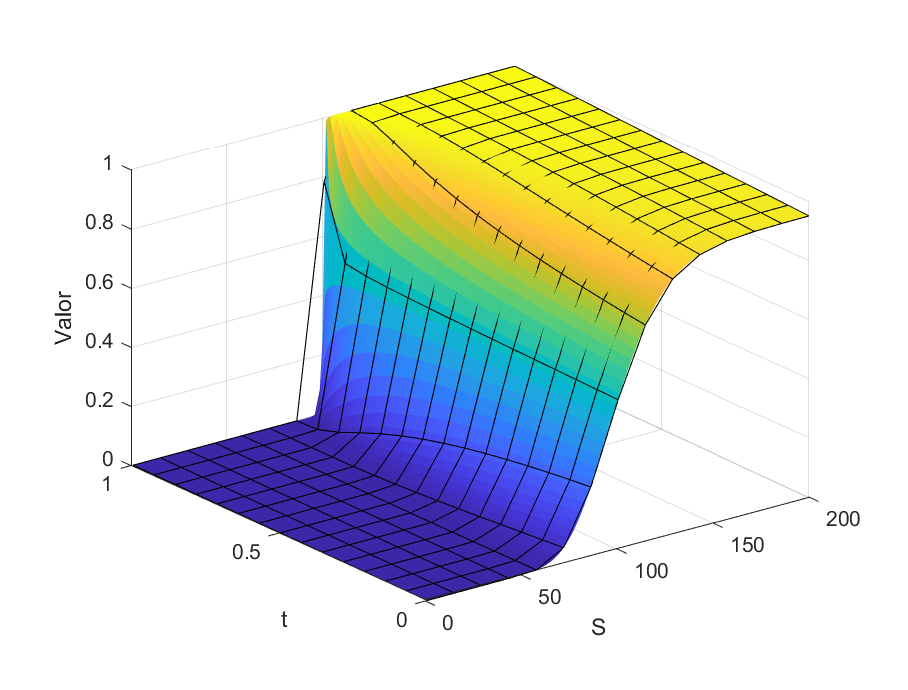
\includegraphics[width=\linewidth]{Imagenes/6_Sols/Binary_Call/BinaryCall3D.eps}
        \caption{Solución}
    \end{subfigure}
    \begin{subfigure}[b]{0.35\linewidth}
        \includegraphics[width=\linewidth]{Imagenes/6_Sols/Binary_Call/BinaryCallSFijo.eps}
        \caption{Solución con S fijo}
    \end{subfigure}
    \begin{subfigure}[b]{0.35\linewidth}
        \includegraphics[width=\linewidth]{Imagenes/6_Sols/Binary_Call/BinaryCalltFIjo.eps}
        \caption{Solución con t fijo}
    \end{subfigure}
    \begin{subfigure}[b]{0.35\linewidth}
        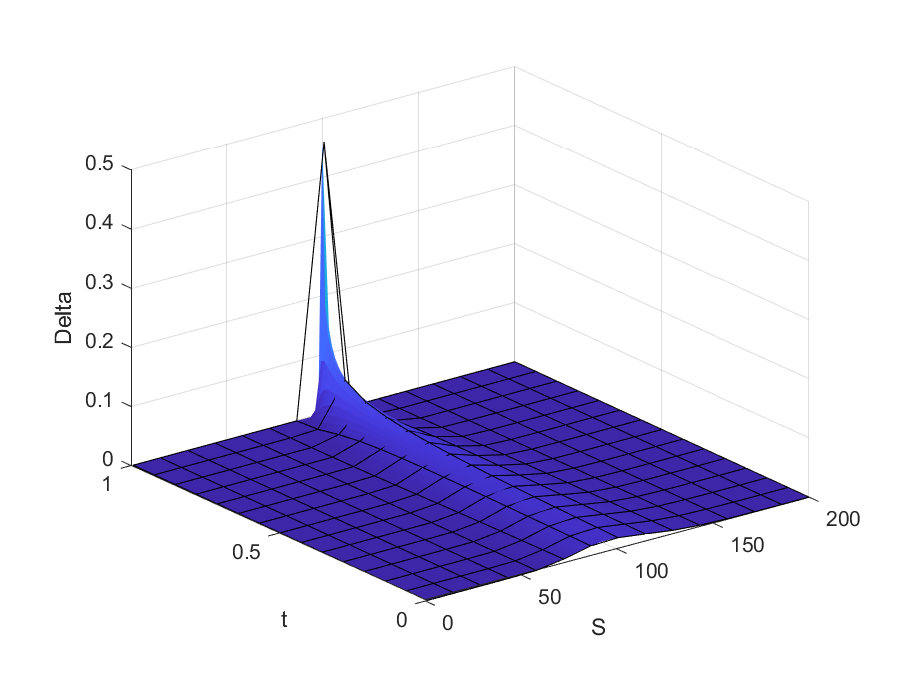
\includegraphics[width=\linewidth]{Imagenes/6_Sols/Binary_Call/Binary_Call_Delta.eps}
        \caption{Delta}
    \end{subfigure}
    \begin{subfigure}[b]{0.35\linewidth}
        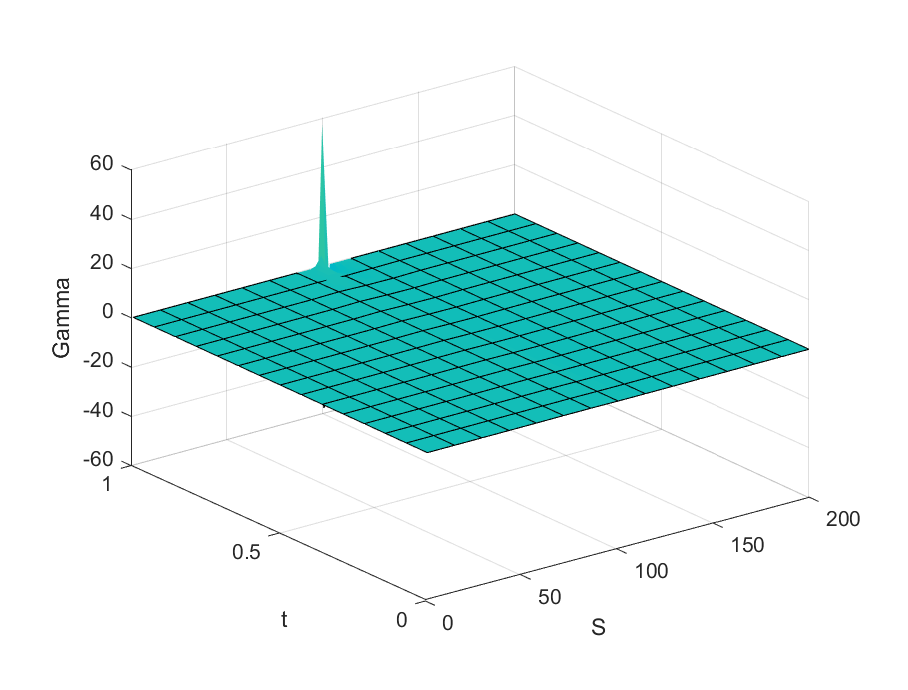
\includegraphics[width=\linewidth]{Imagenes/6_Sols/Binary_Call/Binary_Call_Gamma.eps}
        \caption{Gamma}
    \end{subfigure}
    \begin{subfigure}[b]{0.35\linewidth}
        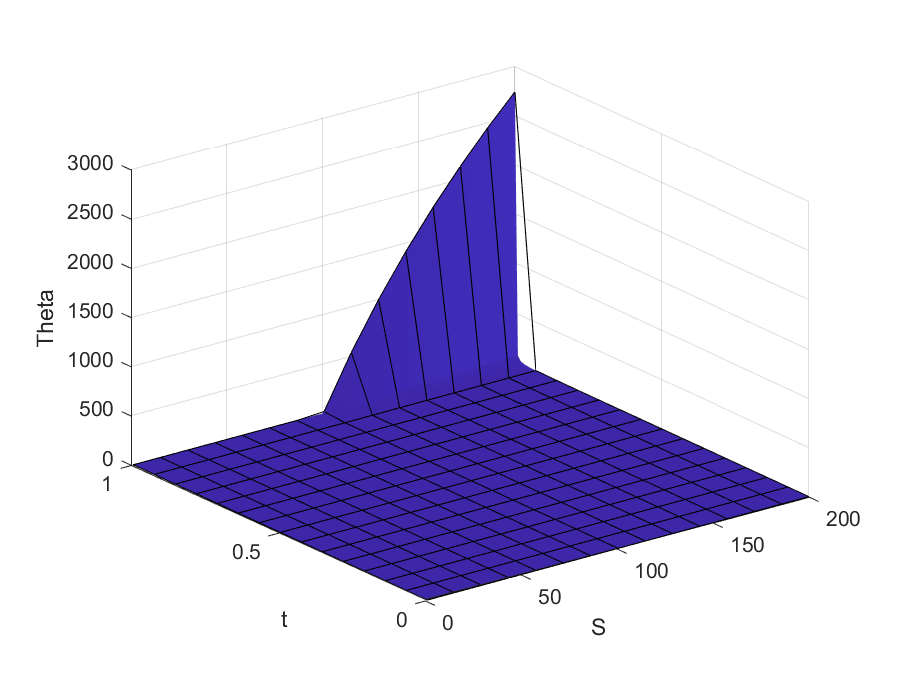
\includegraphics[width=\linewidth]{Imagenes/6_Sols/Binary_Call/Binary_Call_Theta.eps}
        \caption{Theta}
    \end{subfigure}
    \begin{subfigure}[b]{0.35\linewidth}
        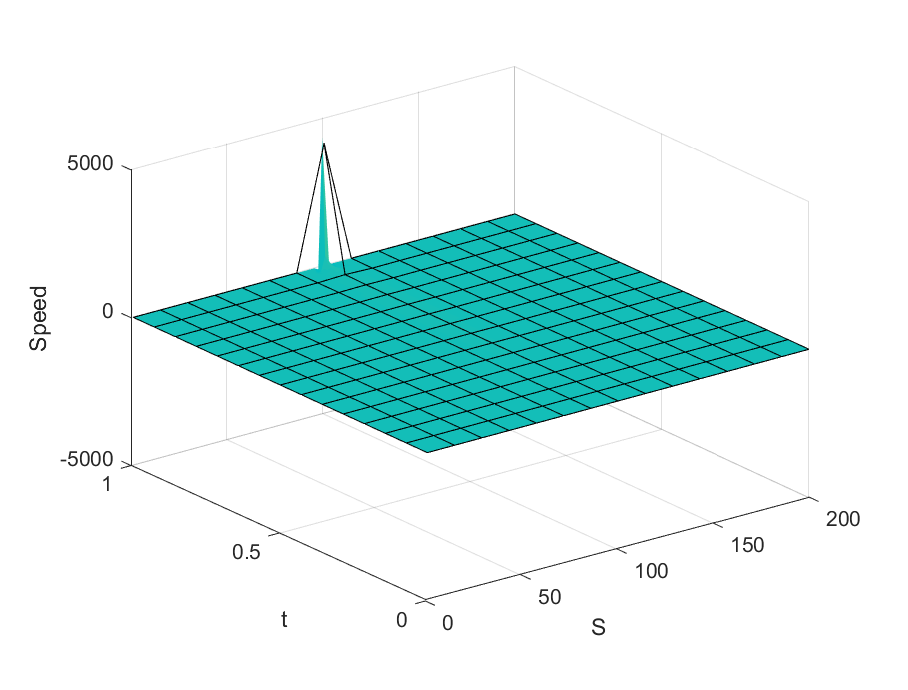
\includegraphics[width=\linewidth]{Imagenes/6_Sols/Binary_Call/Binary_Call_Speed.eps}
        \caption{Speed}
    \end{subfigure}
    \begin{subfigure}[b]{0.35\linewidth}
        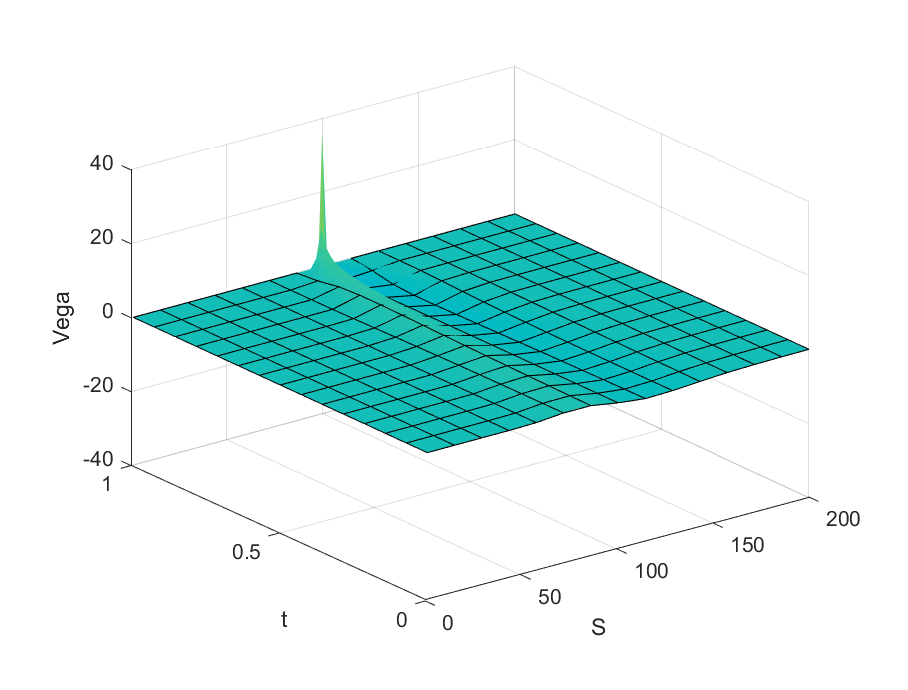
\includegraphics[width=\linewidth]{Imagenes/6_Sols/Binary_Call/Binary_Call_Vega.eps}
        \caption{Vega}
    \end{subfigure}
    \begin{subfigure}[b]{0.35\linewidth}
        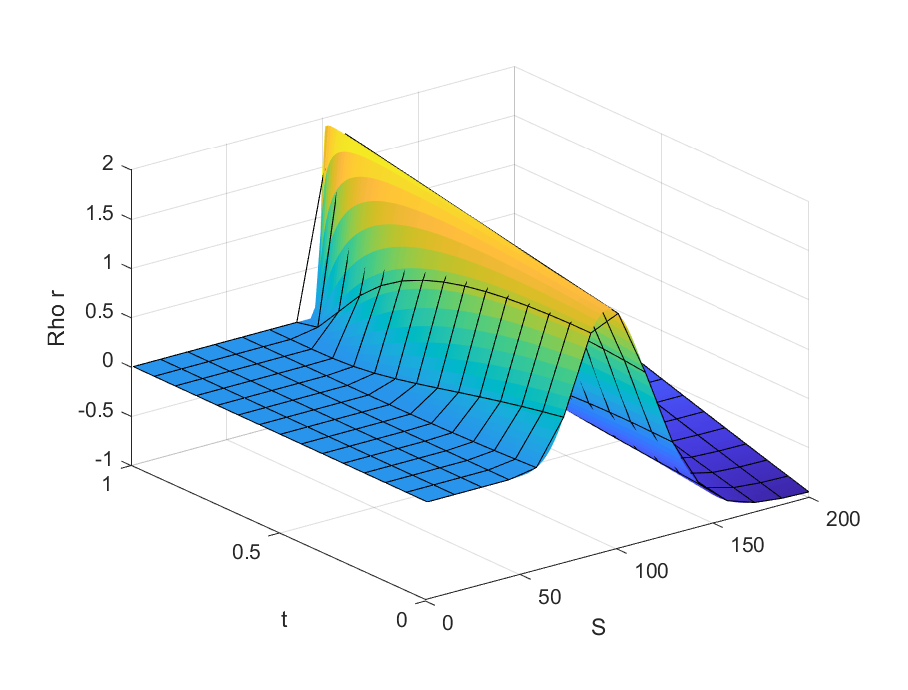
\includegraphics[width=\linewidth]{Imagenes/6_Sols/Binary_Call/Binary_Call_Rho_r.eps}
        \caption{Rho (r)}
    \end{subfigure}
    \begin{subfigure}[b]{0.35\linewidth}
        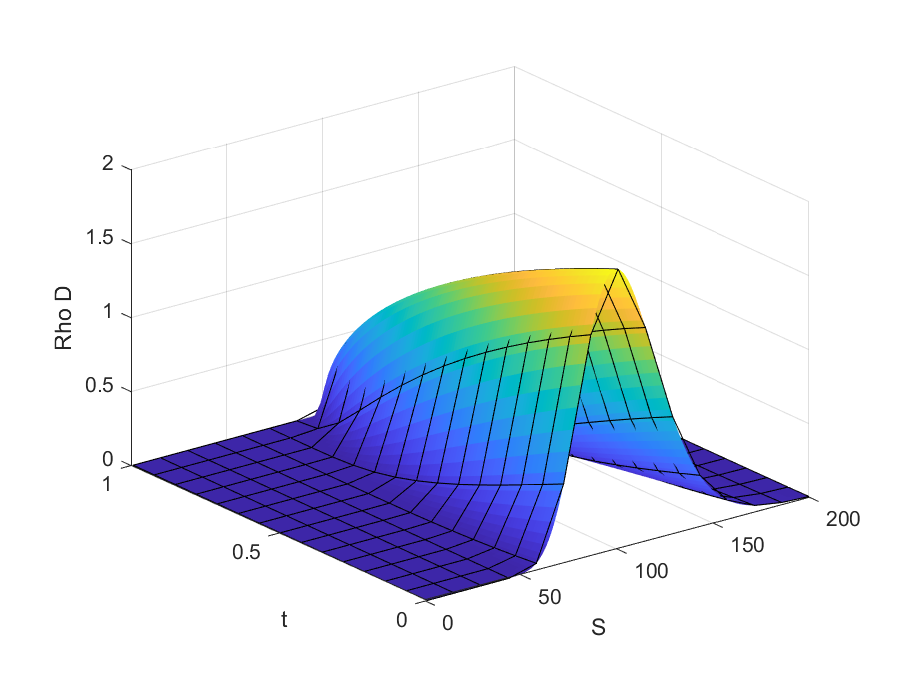
\includegraphics[width=\linewidth]{Imagenes/6_Sols/Binary_Call/Binary_Call_Rho_D.eps}
        \caption{Rho (D)}
    \end{subfigure}
\end{figure}


\subsubsection{Binary Put option}
\begin{figure}[H]
    \centering
    \begin{subfigure}[b]{0.35\linewidth}
        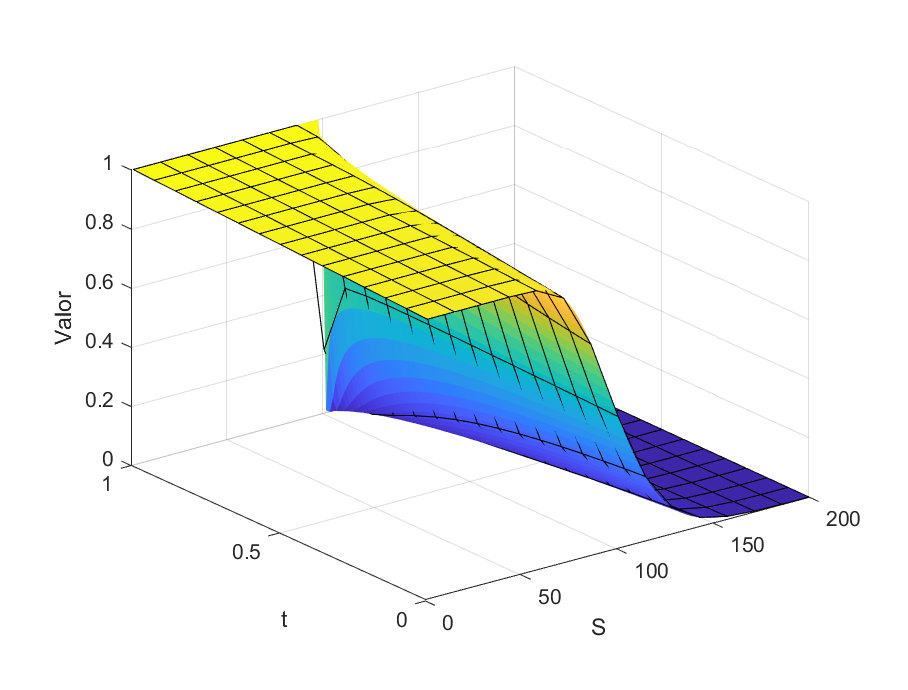
\includegraphics[width=\linewidth]{Imagenes/6_Sols/Binary_Put/BinaryPut3D.eps}
        \caption{Solución}
    \end{subfigure}
    \begin{subfigure}[b]{0.35\linewidth}
        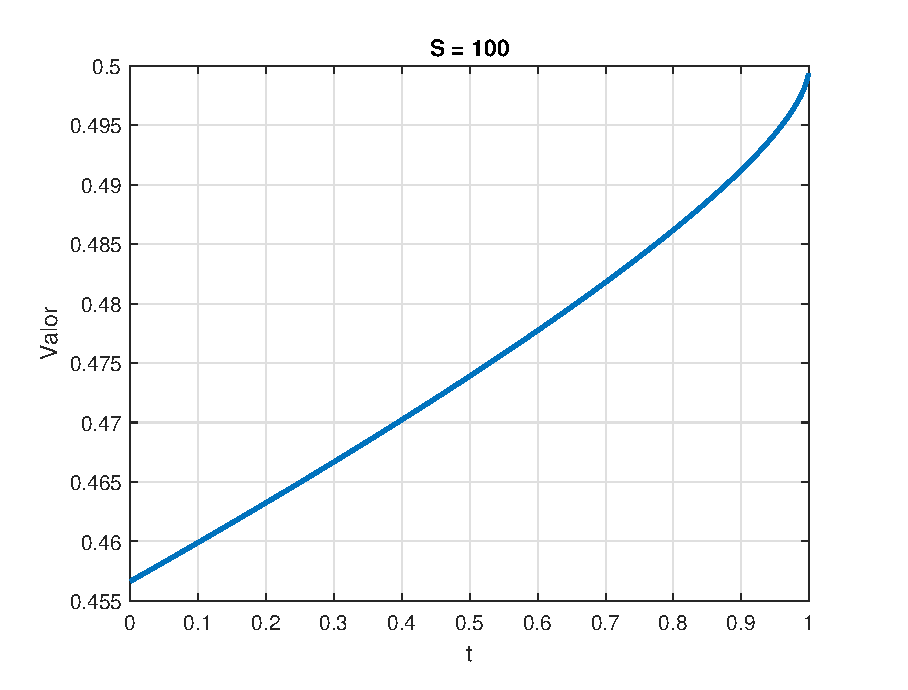
\includegraphics[width=\linewidth]{Imagenes/6_Sols/Binary_Put/BinaryPutSFijo.eps}
        \caption{Solución con S fijo}
    \end{subfigure}
    \begin{subfigure}[b]{0.35\linewidth}
        \includegraphics[width=\linewidth]{Imagenes/6_Sols/Binary_Put/BinaryPuttFIjo.eps}
        \caption{Solución con t fijo}
    \end{subfigure}
    \begin{subfigure}[b]{0.35\linewidth}
        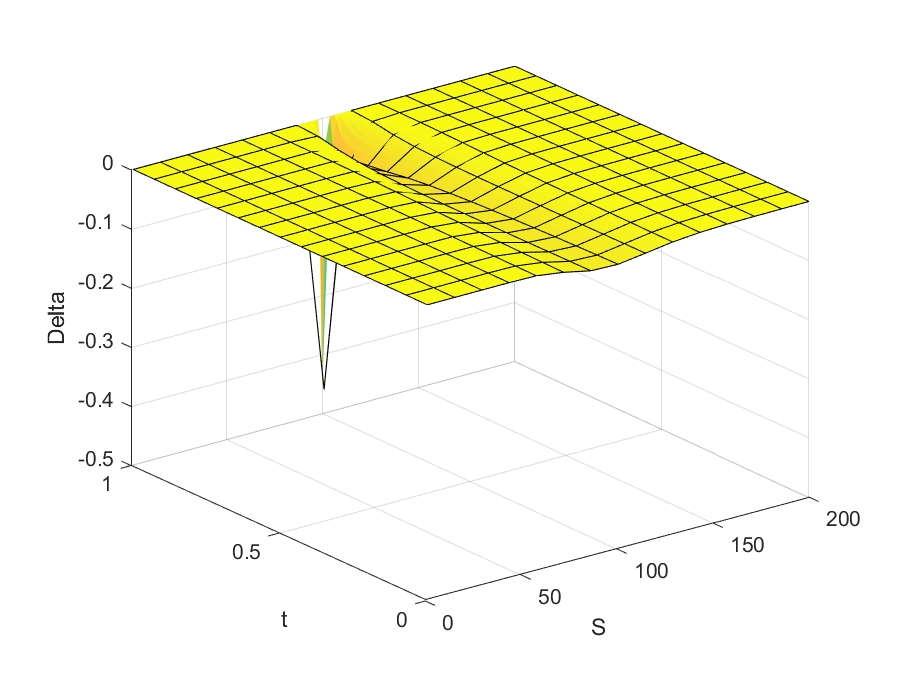
\includegraphics[width=\linewidth]{Imagenes/6_Sols/Binary_Put/Binary_Put_Delta.eps}
        \caption{Delta}
    \end{subfigure}
    \begin{subfigure}[b]{0.35\linewidth}
        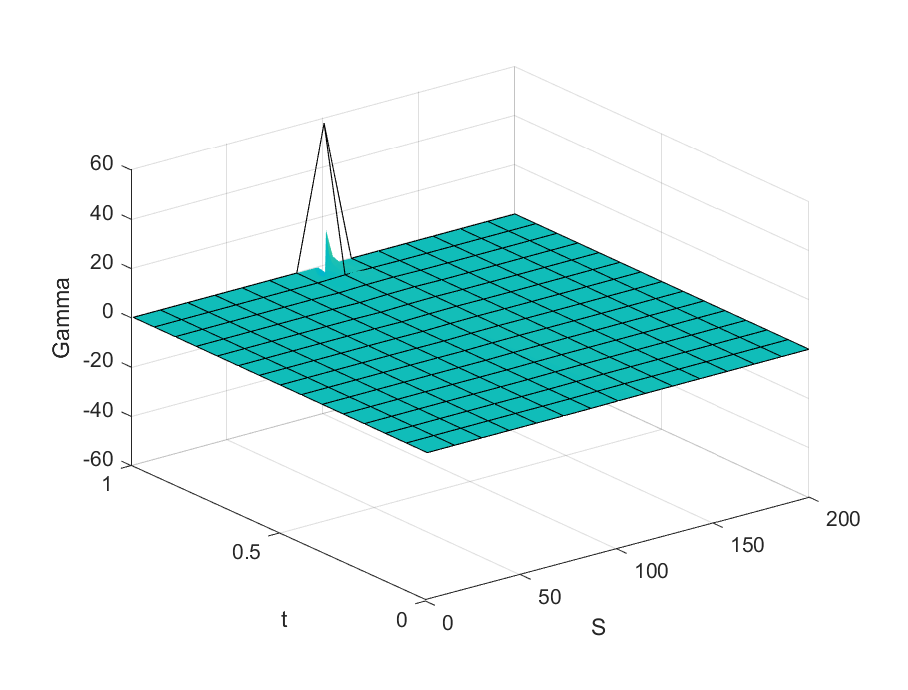
\includegraphics[width=\linewidth]{Imagenes/6_Sols/Binary_Put/Binary_Put_Gamma.eps}
        \caption{Gamma}
    \end{subfigure}
    \begin{subfigure}[b]{0.35\linewidth}
        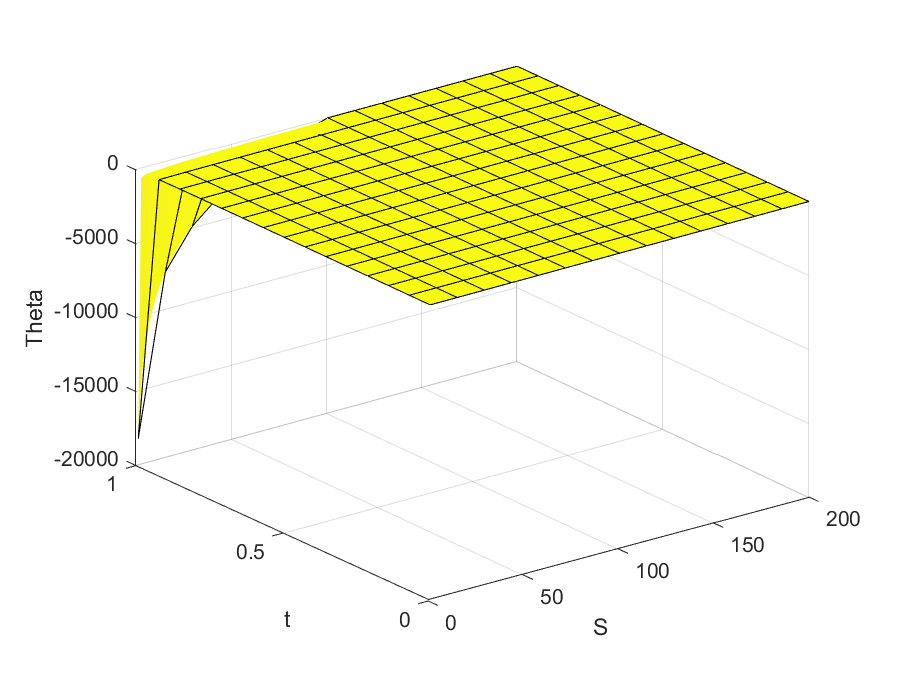
\includegraphics[width=\linewidth]{Imagenes/6_Sols/Binary_Put/Binary_Put_Theta.eps}
        \caption{Theta}
    \end{subfigure}
    \begin{subfigure}[b]{0.35\linewidth}
        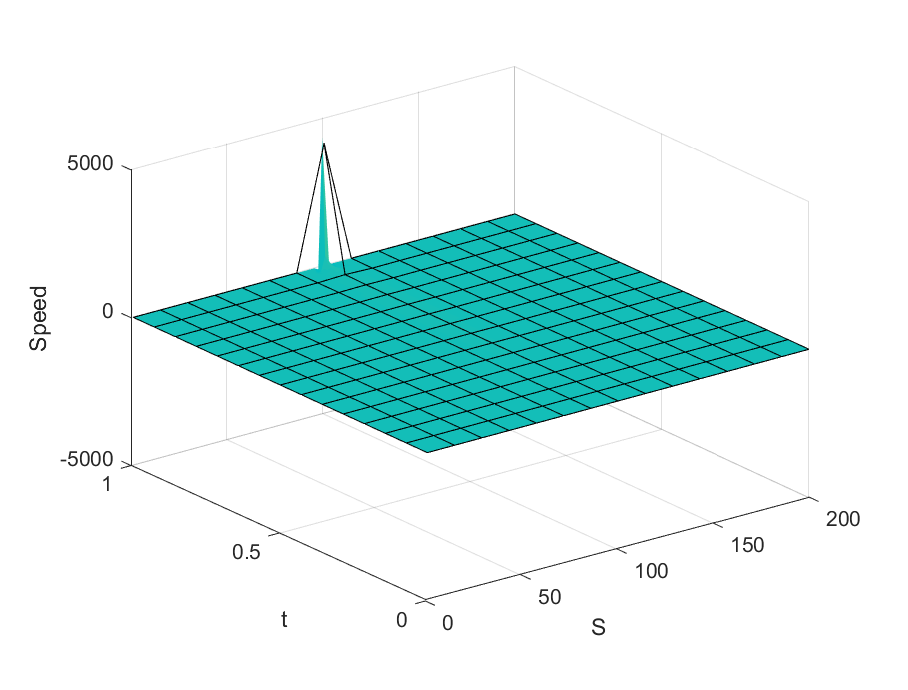
\includegraphics[width=\linewidth]{Imagenes/6_Sols/Binary_Put/Binary_Put_Speed.eps}
        \caption{Speed}
    \end{subfigure}
    \begin{subfigure}[b]{0.35\linewidth}
        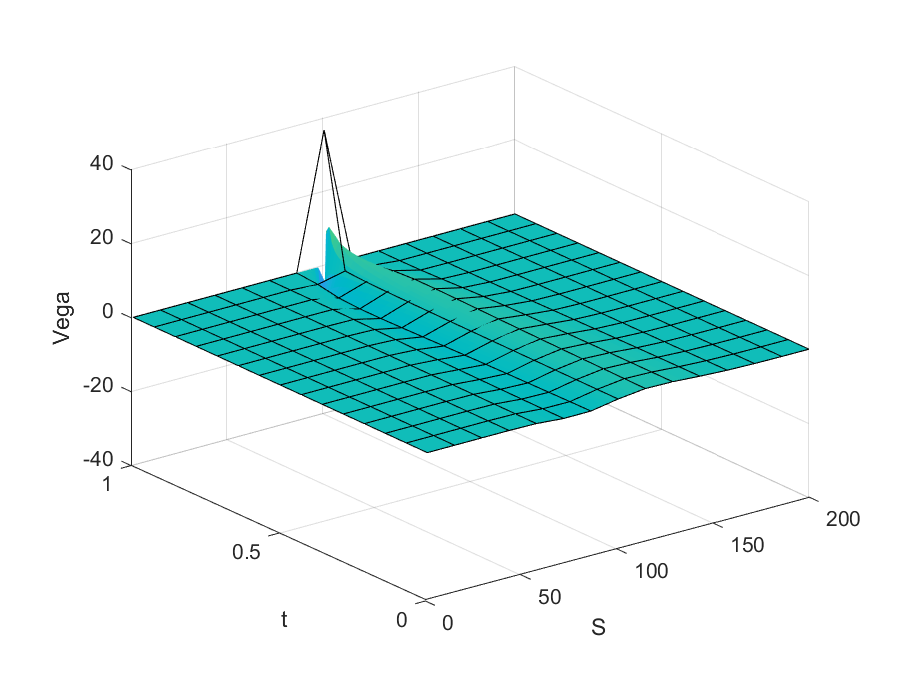
\includegraphics[width=\linewidth]{Imagenes/6_Sols/Binary_Put/Binary_Put_Vega.eps}
        \caption{Vega}
    \end{subfigure}
    \begin{subfigure}[b]{0.35\linewidth}
        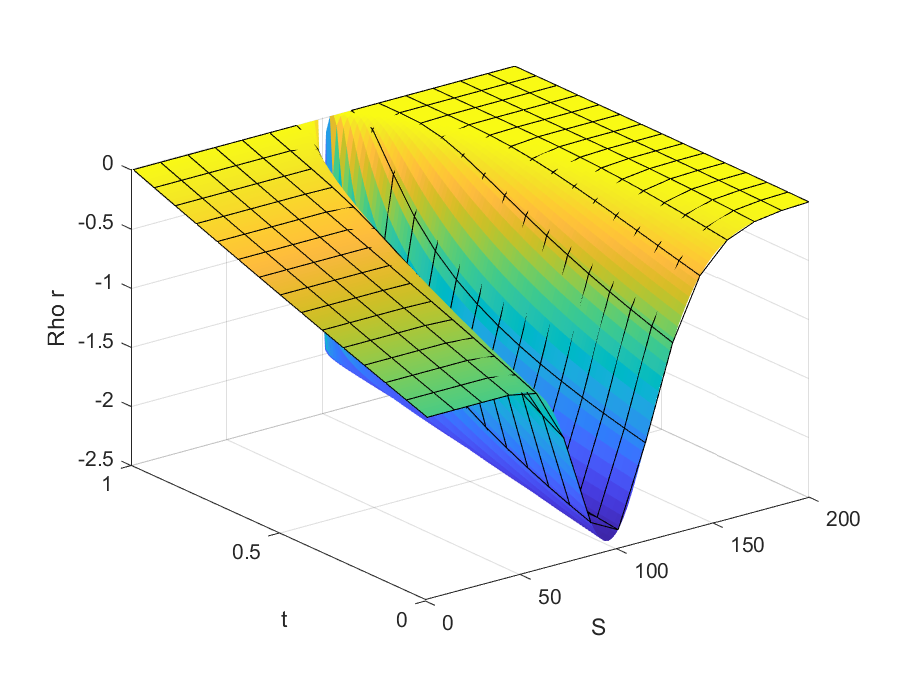
\includegraphics[width=\linewidth]{Imagenes/6_Sols/Binary_Put/Binary_Put_Rho_r.eps}
        \caption{Rho (r)}
    \end{subfigure}
    \begin{subfigure}[b]{0.35\linewidth}
        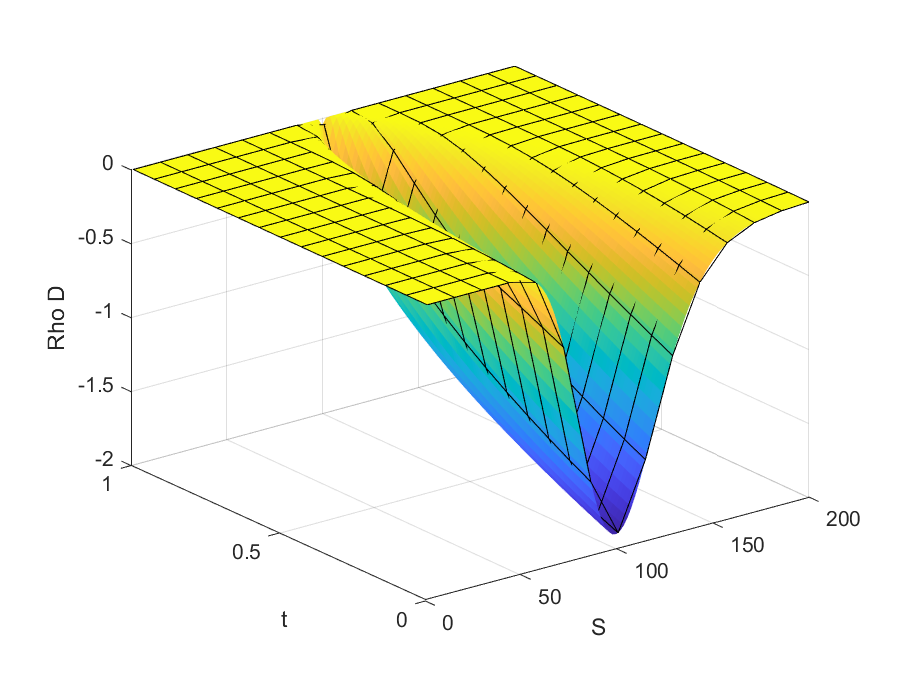
\includegraphics[width=\linewidth]{Imagenes/6_Sols/Binary_Put/Binary_Put_Rho_D.eps}
        \caption{Rho (D)}
    \end{subfigure}
\end{figure}













